\documentclass[crop,tikz]{standalone}

\usepackage{amsmath}

\usetikzlibrary{angles,patterns}
\colorlet{green}{black!40!green}

\begin{document}
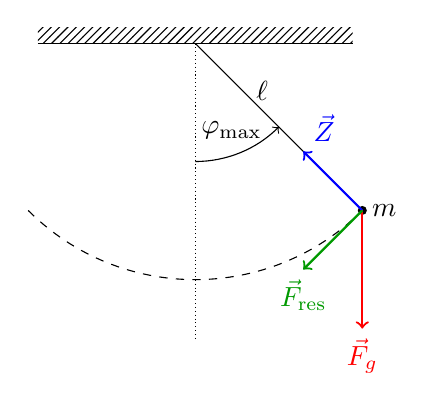
\begin{tikzpicture}
  \pgfmathsetmacro{\Radius}{3};
  \pgfmathsetmacro{\Winkel}{1.5*30};
  \pgfmathsetmacro{\mass}{1};
  \pgfmathsetmacro{\gerde}{1.5};
  \pgfmathsetmacro{\mg}{\mass*\gerde};
  %
  \coordinate (O) at (0,0);
  \coordinate (N) at (0,{-\Radius});
  \coordinate (M) at ({270+\Winkel}:{\Radius});
  %
  \pattern[pattern=north east lines,pattern color=black] (-2,0) rectangle (2,0.2);
  \draw (-2,0) -- (2,0);
  \draw[densely dotted] (O) -- (0,{-1.25*\Radius});
  \draw[dashed] ({270-\Winkel}:{\Radius}) arc ({270-\Winkel}:{270+\Winkel}:{\Radius});
  % mass
  \draw[fill] (M) circle (0.05) node[right] {$m$};
  \draw (O) -- node[pos=0.4,above] {$\ell$} (M);
  \pic[draw,->,angle eccentricity=0.8,angle radius=1.5cm,pic text={$\varphi_{\max}$}] {angle = N--O--M};
  % gravity
  \draw[->,red,thick] (M) -- ++ (0,{-\mg}) node[below] {$\vec{F}_g$}; 
  % string force
  \draw[->,blue,thick] (M) -- ++ ({\Winkel+90}:{\mg*cos(\Winkel)}) node[above right] {$\vec{Z}$};
  % resulting force
  \draw[->,green,thick] (M) -- ++ ({\Winkel+180}:{\mg*sin(\Winkel)}) node[below] {$\vec{F}_{\text{res}}$};
\end{tikzpicture}
\end{document}
